\section{Serial Data Transfer - UART \& I2C}

\subsection{UART Fundamentals}

\mult{2}

\begin{concept}{UART - Universal Asynchronous Receiver Transmitter}\\
UART is an asynchronous serial communication interface:
\begin{itemize}
    \item Asynchronous - no shared clock between transmitter and receiver
    \item Point-to-point communication (one transmitter, one receiver)
    \item Full-duplex (simultaneous bidirectional communication)
    \item Start and stop bits used for synchronization
    \item Typically 2-wire interface (TX and RX) for data
    \item Optional control signals (RTS/CTS, etc.) for flow control
\end{itemize}
\end{concept}

\begin{definition}{UART Signals}\\
Basic UART connections require:
\begin{itemize}
    \item \textbf{TX} (Transmit): Data output from transmitter to receiver
    \item \textbf{RX} (Receive): Data input from transmitter to receiver
    \item \textbf{GND} (Ground): Common reference level
\end{itemize}
Extended UART (with hardware flow control) may include:
\begin{itemize}
    \item \textbf{RTS} (Request to Send): Output indicating readiness to receive
    \item \textbf{CTS} (Clear to Send): Input indicating partner is ready to receive
\end{itemize}
\end{definition}

\multend

\subsection{UART Data Format and Timing}

\mult{2}

\begin{definition}{UART Frame Structure}\\
A UART frame consists of:
\begin{itemize}
    \item \textbf{Idle state}: Line is high ('1') when no transmission occurs
    \item \textbf{Start bit}: Always '0', indicates beginning of frame
    \item \textbf{Data bits}: 5 to 9 bits (typically 8), LSB first
    \item \textbf{Parity bit} (optional): For error detection
    \item \textbf{Stop bit(s)}: 1, 1.5, or 2 bits, always '1'
\end{itemize}
\end{definition}

\begin{concept}{UART Synchronization}\\
Without a common clock, UART devices synchronize as follows:
\begin{itemize}
    \item Receiver detects start bit (falling edge from idle to '0')
    \item Receiver samples middle of each bit based on configured baud rate
    \item Both devices must use the same configuration:
    \begin{itemize}
        \item Baud rate (e.g., 9600, 115200 bits/s)
        \item Number of data bits (5-8)
        \item Parity (none, odd, even, mark, space)
        \item Number of stop bits (1, 1.5, 2)
    \end{itemize}
\end{itemize}
\end{concept}

\begin{example2}{UART Timing Diagram Analysis}\\
Given a UART signal with 8 data bits, no parity, 1 stop bit, analyze this pattern:
\\
$\overline{\text{\_\_\_\_\_}}$ $\overline{\text{\_\_}}$ $\overline{\text{\_\_\_\_}}$ $\overline{\text{\_\_}}$ $\overline{\text{\_\_\_\_}}$ $\overline{\text{\_\_\_\_\_\_\_\_\_\_}}$
\\
I I S D D D D D D D D E I I
\\
Where I=Idle, S=Start, D=Data, E=Stop
\tcblower
Breaking down this signal:
- Idle (high) $\rightarrow$ Start bit (low) $\rightarrow$ 8 data bits $\rightarrow$ Stop bit (high) $\rightarrow$ Idle (high)
- Reading data bits (LSB first): 01010011
- Converting to binary: 0b01010011 = 0x53 = ASCII 'S'

This UART transmission contains the character 'S'.
\end{example2}

\begin{formula}{UART Calculations}\\
\textbf{Bit Time (seconds):}
$T_{bit} = \frac{1}{\text{Baud Rate}}$


\textbf{Frame Time (seconds):}
$T_{frame} =$\\$T_{bit} \times (1 + \text{Data Bits} + \text{Parity Bits} + \text{Stop Bits})$


\textbf{Maximum Data Rate (bytes/second):}\\
$\text{Data Rate} = \frac{\text{Baud Rate}}{\text{Total Bits per Byte}}$

where Total Bits per Byte = 1 (start) + Data Bits + Parity Bits + Stop Bits
\end{formula}

\begin{KR}{Clock Tolerance in UART}
\paragraph{Maximum clock deviation}
The receiver must sample correctly until the last bit:
\paragraph{Formula}
Maximum allowed clock deviation (as percentage):
$\text{Deviation}_{\max} = \frac{0.5}{N} \times 100\%$

where N is the number of bit times between synchronization points.
\end{KR}

\begin{example}
    For a standard UART frame (1 start, 8 data, 1 stop):\\
    Synchronization occurs at start bit,
    Last bit (stop bit) is 10 bits later\\
    Maximum clock deviation = 0.5/10 = 5\%\\
    Sample calculation:\\
    If sender clock is 9600 Hz: Receiver can be between 9120 Hz and 10080 Hz
\end{example}

\multend


\subsection{UART on STM32F4}

\begin{concept}{STM32F4 UART/USART Peripherals}\\
The STM32F4 includes several UART/USART modules with features:
\begin{itemize}
    \item Full-duplex communication (USART)
    \item Programmable baud rate
    \item Configurable data bits, stop bits, and parity
    \item Interrupt generation on events (TX empty, RX not empty, etc.)
    \item DMA support for efficient data transfer
    \item Hardware flow control (CTS/RTS) on USARTs
    \item Synchronous mode available on USARTs
\end{itemize}
\end{concept}

\begin{code}{STM32F4 UART Configuration} Configure UART2 for 115200 baud, 8-N-1
\begin{lstlisting}[language=C, style=basesmol]
// 1. Enable UART2 and GPIO clock
RCC->APB1ENR |= RCC_APB1ENR_USART2EN;  // Enable UART2 clock
RCC->AHB1ENR |= RCC_AHB1ENR_GPIOAEN;   // Enable GPIOA clock
// 2. Configure GPIO pins for UART (PA2 = TX, PA3 = RX)
// Set alternate function mode (0x10)
GPIOA->MODER &= ~(0x3 << (2*2) | 0x3 << (2*3));
GPIOA->MODER |= (0x2 << (2*2) | 0x2 << (2*3));
// Set to AF7 (UART2)
GPIOA->AFR[0] &= ~(0xF << (4*2) | 0xF << (4*3));
GPIOA->AFR[0] |= (0x7 << (4*2) | 0x7 << (4*3));
// 3. Configure UART
// Reset UART configuration
USART2->CR1 = 0;
USART2->CR2 = 0;
USART2->CR3 = 0;
// Set baud rate (assuming 84MHz APB1 clock)
// BRR = f_CK / baud rate = 84,000,000 / 115,200 = 729.16
USART2->BRR = 729;
// Enable UART, TX, and RX
USART2->CR1 = USART_CR1_UE | USART_CR1_TE | USART_CR1_RE;
\end{lstlisting}
\end{code}

\begin{KR}{UART Data Transmission and Reception}
\textbf{Transmitting Data}
Write data to the data register after checking the TXE flag.\\
\textbf{Receiving Data}
Read from the data register after checking the RXNE flag.

\begin{lstlisting}[language=C, style=basesmol]
// Send a character
void UART_SendChar(USART_TypeDef *uart, char c) {
    // Wait until TXE flag is set (transmit buffer empty)
    while (!(uart->SR & USART_SR_TXE)) { }
    // Write the character to the data register
    uart->DR = c;
}
// Send a string
void UART_SendString(USART_TypeDef *uart, const char *str) {
    while (*str) {
        UART_SendChar(uart, *str++);
    }
}
// Receive a character (blocking)
char UART_ReceiveChar(USART_TypeDef *uart) {
    // Wait until RXNE flag is set (data received)
    while (!(uart->SR & USART_SR_RXNE)) { }
    // Return received data
    return uart->DR;
}
\end{lstlisting}
\end{KR}


\subsection{I2C Fundamentals}

\begin{concept}{I2C - Inter-Integrated Circuit}\\
I2C is a synchronous, half-duplex, multi-master bus:
\begin{itemize}
    \item Developed by Philips (now NXP) in 1982
    \item 2-wire interface (SCL and SDA)
    \item Multi-master, multi-slave capability
    \item Unique 7-bit or 10-bit address for each device
    \item Synchronous (master provides clock)
    \item Half-duplex (data flows in one direction at a time)
    \item Well-suited for connecting multiple boards or chips
    \item Bit rates from 100 kbit/s (standard) to 5 Mbit/s (ultra-fast)
\end{itemize}
\end{concept}

\begin{definition}{I2C Signals}\\
I2C requires just two bidirectional lines with pull-up resistors:
\begin{itemize}
    \item \textbf{SCL} (Serial Clock Line): Clock signal generated by master
    \item \textbf{SDA} (Serial Data Line): Bidirectional data line
\end{itemize}
Both lines are open-drain, requiring external pull-up resistors.
\end{definition}

\subsection{I2C Protocol}

\begin{concept}{I2C Bus Conditions}\\
Special conditions on the I2C bus:
\begin{itemize}
    \item \textbf{START condition}: SDA goes from high to low while SCL is high
    \item \textbf{STOP condition}: SDA goes from low to high while SCL is high
    \item \textbf{Data valid}: SDA remains stable while SCL is high
    \item \textbf{Data change}: SDA changes only when SCL is low
\end{itemize}
\end{concept}

\begin{definition}{I2C Data Transfer}\\
Data transfer sequence:
\begin{itemize}
    \item Master initiates transfer with START condition
    \item Master sends 7-bit slave address + R/W bit (0 = write, 1 = read)
    \item Addressed slave acknowledges (ACK) by pulling SDA low
    \item Data bytes transferred (8 bits followed by ACK/NACK)
    \item Master terminates transfer with STOP condition
\end{itemize}
Data is transferred MSB first, with the receiver acknowledging each byte.
\end{definition}

\begin{concept}{I2C Acknowledge and Not-Acknowledge}\\
After each byte transfer:
\begin{itemize}
    \item \textbf{ACK} (Acknowledge): Receiver pulls SDA low during 9th clock cycle
    \item \textbf{NACK} (Not-Acknowledge): SDA remains high during 9th clock cycle
\end{itemize}
NACK can indicate:
\begin{itemize}
    \item No receiver with the transmitted address
    \item Receiver unable to receive or transmit
    \item Receiver doesn't understand the data/command
    \item Receiver cannot receive more data
    \item Master-receiver signals end of transfer to slave-transmitter
\end{itemize}
\end{concept}

\begin{example2}{I2C Write Operation}\\
Master wants to write data 0x9C to slave with address 0x66
\tcblower
1. Master generates START condition
2. Master sends slave address (0x66) with R/W = 0 (write): 0xCC
3. Slave acknowledges (ACK)
4. Master sends data byte 0x9C
5. Slave acknowledges (ACK)
6. Master generates STOP condition

I2C bus:
START - 0xCC - ACK - 0x9C - ACK - STOP
\end{example2}

\begin{example2}{I2C Read Operation}\\
Master wants to read data from slave with address 0x66
\tcblower
1. Master generates START condition
2. Master sends slave address (0x66) with R/W = 1 (read): 0xCD
3. Slave acknowledges (ACK)
4. Slave sends data byte (e.g., 0x9C)
5. Master sends NACK to indicate end of transfer
6. Master generates STOP condition

I2C bus:
START - 0xCD - ACK - 0x9C - NACK - STOP
\end{example2}

\subsection{I2C on STM32F4}

\begin{concept}{STM32F4 I2C Peripherals}\\
The STM32F4 includes I2C modules with features:
\begin{itemize}
    \item Compatible with I2C standard protocol
    \item Multiple speed modes (standard, fast)
    \item 7-bit and 10-bit addressing
    \item Multi-master capability
    \item Programmable clock stretching
    \item Programmable NOSTRETCH capability
    \item DMA support for efficient data transfer
    \item SMBus support
\end{itemize}
\end{concept}

\begin{code}{STM32F4 I2C Configuration}
\begin{lstlisting}[language=C, style=basesmol]
// Configure I2C1 for 100kHz standard mode

// 1. Enable I2C1 and GPIO clock
RCC->APB1ENR |= RCC_APB1ENR_I2C1EN;   // Enable I2C1 clock
RCC->AHB1ENR |= RCC_AHB1ENR_GPIOBEN;  // Enable GPIOB clock

// 2. Configure GPIO pins for I2C (PB6 = SCL, PB7 = SDA)
// Set alternate function mode (0x10)
GPIOB->MODER &= ~(0x3 << (2*6) | 0x3 << (2*7));
GPIOB->MODER |= (0x2 << (2*6) | 0x2 << (2*7));

// Set open-drain output type
GPIOB->OTYPER |= (1 << 6) | (1 << 7);

// Set to AF4 (I2C1)
GPIOB->AFR[0] &= ~(0xF << (4*6) | 0xF << (4*7));
GPIOB->AFR[0] |= (0x4 << (4*6) | 0x4 << (4*7));

// 3. Reset I2C
I2C1->CR1 = I2C_CR1_SWRST;  // Software reset
I2C1->CR1 = 0;              // Clear reset

// 4. Configure I2C
// Set peripheral clock frequency (42MHz)
I2C1->CR2 = 42;  // FREQ = 42MHz

// Set CCR for 100kHz standard mode
// CCR = PCLK1 / (2 * I2C_FREQ) = 42MHz / (2 * 100kHz) = 210
I2C1->CCR = 210;

// Set TRISE
// TRISE = (max rise time * PCLK1) + 1 = (1000ns * 42MHz) + 1 = 43
I2C1->TRISE = 43;

// 5. Enable I2C
I2C1->CR1 |= I2C_CR1_PE;  // Peripheral enable
\end{lstlisting}
\end{code}

\begin{KR}{I2C Master Transmit and Receive}
\paragraph{Master Transmit Sequence}
Generate START, send address+write, send data bytes, generate STOP.
\paragraph{Master Receive Sequence}
Generate START, send address+read, receive data bytes with ACK/NACK, generate STOP.

\begin{lstlisting}[language=C, style=basesmol]
// I2C Master Transmit
void I2C_MasterTransmit(I2C_TypeDef *i2c, uint8_t address, uint8_t *data, uint16_t size) {
    // 1. Wait until I2C bus is free
    while (i2c->SR2 & I2C_SR2_BUSY) { }
    
    // 2. Generate START condition
    i2c->CR1 |= I2C_CR1_START;
    
    // 3. Wait for EV5 (START sent)
    while (!(i2c->SR1 & I2C_SR1_SB)) { }
    
    // 4. Send slave address (write mode)
    i2c->DR = address << 1;  // Address + Write bit (0)
    
    // 5. Wait for EV6 (address sent)
    while (!(i2c->SR1 & I2C_SR1_ADDR)) { }
    
    // 6. Clear ADDR by reading SR2
    (void)i2c->SR2;
    
    // 7. Send data bytes
    for (uint16_t i = 0; i < size; i++) {
        // Wait until TXE is set
        while (!(i2c->SR1 & I2C_SR1_TXE)) { }
        
        // Send data byte
        i2c->DR = data[i];
    }
    
    // 8. Wait for transfer to complete
    while (!(i2c->SR1 & I2C_SR1_TXE) || !(i2c->SR1 & I2C_SR1_BTF)) { }
    
    // 9. Generate STOP condition
    i2c->CR1 |= I2C_CR1_STOP;
}
\end{lstlisting}
\end{KR}

\subsection{Comparison of Serial Interfaces}

\begin{concept}{UART vs. SPI vs. I2C Comparison}
\begin{center}
\begin{tabular}{|p{2.5cm}|p{4cm}|p{4cm}|p{4cm}|}
\hline
\textbf{Feature} & \textbf{UART} & \textbf{SPI} & \textbf{I2C} \\
\hline
Wires & 2 (TX, RX) & 4 (MOSI, MISO, SCLK, SS) & 2 (SDA, SCL) \\
\hline
Clock & Asynchronous & Synchronous & Synchronous \\
\hline
Connection Type & Point-to-point & Point-to-multipoint & Multi-point \\
\hline
Duplex & Full-duplex & Full-duplex & Half-duplex \\
\hline
Addressing & Higher layer only & Device selection via SS & 7/10-bit addressing \\
\hline
Error Detection & Optional parity bit & None & ACK/NACK \\
\hline
Speed & Up to ~5 Mbps & Up to ~50 Mbps & 100 kbps to 5 Mbps \\
\hline
Master/Slave & Peer-to-peer & Single master, multiple slaves & Multiple masters, multiple slaves \\
\hline
Typical Use & Terminal communication, debug ports & On-board high-speed communication & Board-to-board, chip-to-chip \\
\hline
\end{tabular}
\end{center}
\end{concept}

\section{Serial Data Transfer}

\begin{concept}{Overview}\\
    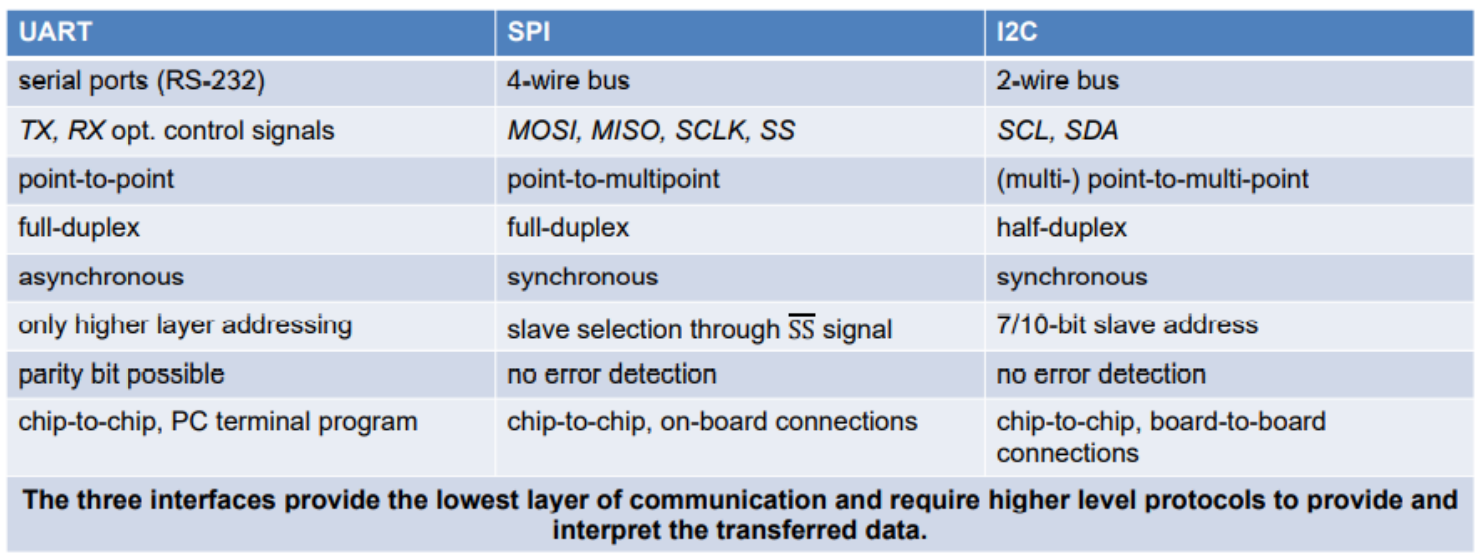
\includegraphics[width=\linewidth]{SDT_overview.png}
    \vspace{2mm}\\
    \textbf{SPI - Serial Peripheral Interface}
    \begin{itemize}
        \item Master/slave
        \item Synchronous full-duplex transmissions (MOSI, MISO)
        \item Selection of device through Slave Select (SS)
        \item no acknowledge, no error detection
        \item Clock signal (SCK) for synchronization: four mode $\rightarrow$ CPOL (clock polarity), CPHA (clock phase)
    \end{itemize}
    \vspace{2mm}

    \textbf{UART - Universal Asynchronous Receiver Transmitter} (Serial Interface)
    \begin{itemize}
        \item Transmitter and receiver use diverging clocks
        \item synchronization using start and stop bits $\rightarrow$ overhead
        \item longer connections require line drivers $\rightarrow$ RS-232/RS-485
    \end{itemize}
    \vspace{2mm}

    \textbf{I2C - Inter-Integrated Circuit}
    \begin{itemize}
        \item Synchronous half-duplex transmission (SCL, SDA)
        \item 7-bit slave addresses
        \item Acknowledge, error detection
        \item Clock signal (SCL) for synchronization
    \end{itemize}
\end{concept}

\begin{definition}{Single Master - Multiple Slaves}
    \begin{itemize}
        \item Master generates a common clock signal for all Slaves
        \item MOSI: From Master Output to all Slave Inputs
        \item MISO: From Master Input to all Slave Outputs $\rightarrow$ all slave outpuzs connected to single master input
        \item Slaves: Selectable by Slave Select (SS) signal
        \begin{itemize}
            \item Individual Select $\overline{SS1}$, $\overline{SS2}$, $\overline{SS3}$
            \item $\overline{SSx}$ = 1 $\rightarrow$ slave output MISOx is tri-state 
        \end{itemize}
    \end{itemize}
    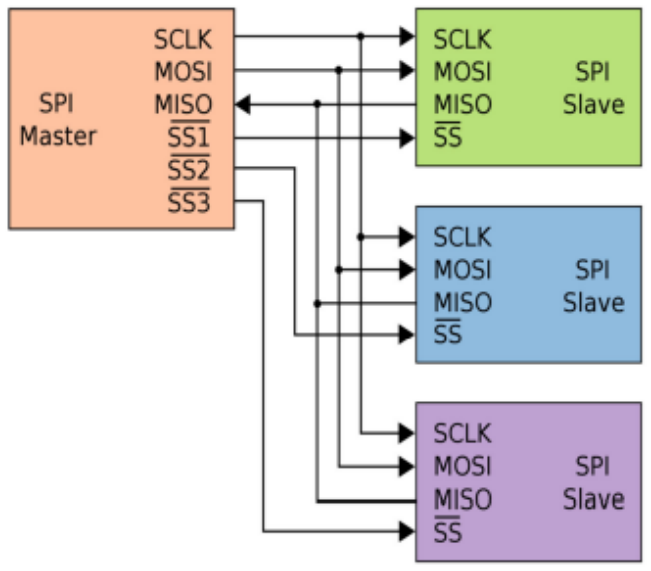
\includegraphics[width=\linewidth]{single_master_mult_slaves.png}
\end{definition}

\begin{formula}{Clock Polarity (CPOL) Clock Phase (CPHA)}
    \begin{itemize}
        \item \textbf{CPOL:} Clock Polarity
        \begin{itemize}
            \item 0: Clock is low in idle state
            \item 1: Clock is high in idle state
        \end{itemize}
        \item \textbf{CPHA:} Clock Phase
        \begin{itemize}
            \item 0: Data is sampled on the first edge of the clock
            \item 1: Data is sampled on the second edge of the clock
        \end{itemize}
    \end{itemize}
    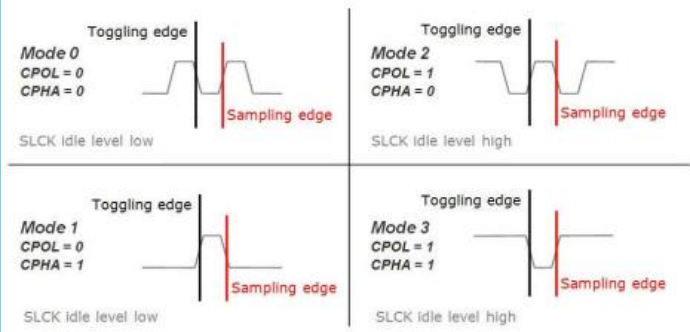
\includegraphics[width=\linewidth]{clockpolarity.png}
    \begin{itemize}
        \item TX provides data on \oq Toggling Edge\cq
        \item RX takes over data with \oq Sampling Edge\cq
    \end{itemize}
\end{formula}

\subsection{Serial Connection - SPI}

\begin{definition}{Properties of SPI}
    \begin{itemize}
        \item No defined addressing scheme
        \begin{itemize}
            \item Use of $\overline{SS}$ instead $\rightarrow$ KISS (Keep It Simple Stupid)
        \end{itemize}
        \item Transmission without receive acknowledge and error detection
        \begin{itemize}
            \item Has to be implemented in higher level protocols
        \end{itemize}
        \item Originally used only for transmission of single bytes
        \begin{itemize}
            \item $\overline{SS}$ deactivated after each byte
            \item Today also used for streams 
        \end{itemize}
        \item Data rate: Highly flexible as clock signal is transmitted
        \item No flow-control available
        \begin{itemize}
            \item Master can delay the next clock edge
            \item Slave can't influence the data rate
        \end{itemize}
        \item Susceptible to noise (spikes on clock signal)
    \end{itemize}
\end{definition}

\begin{example2}{SPI - Serial Peripheral Interface}\\
    Ein Prozessor (SPI Master) sendet das Byte 0x3D = 0011 1101\\
    Die Schnittstelle ist wie folgt konfiguriert:\\
    Mode = 3, CPOL = 1, CPHA = 1, MSB first\\
    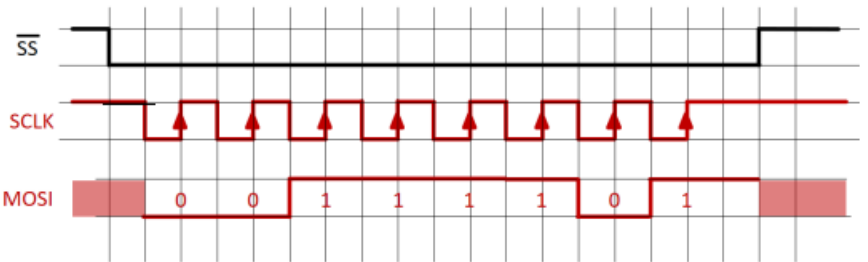
\includegraphics[width=\linewidth]{spi_example.png}
\end{example2}

\begin{concept}{Synchronizing Hardware and Software}
    \begin{itemize}
        \item TXE (TX Buffer Empty) $\rightarrow$ Software can write next TX Byte to SPI\_DR
        \item RXNE (RX Buffer Not Empty) $\rightarrow$ a byte has been received. Software can read it from SPI\_DR
        \item BSY (Busy) $\rightarrow$ Transmission in progress
    \end{itemize}
    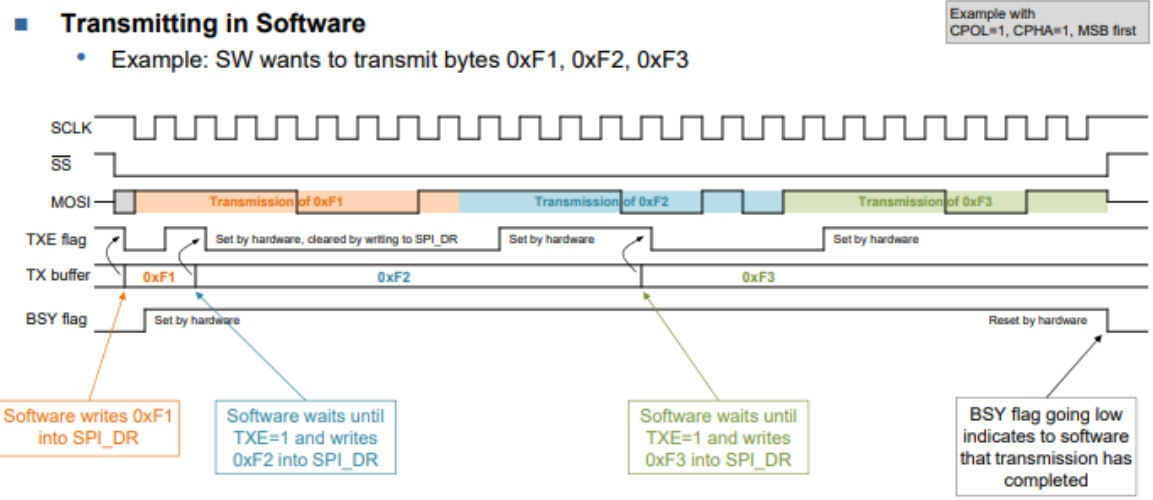
\includegraphics[width=\linewidth]{transmitting_spi.png}\\
    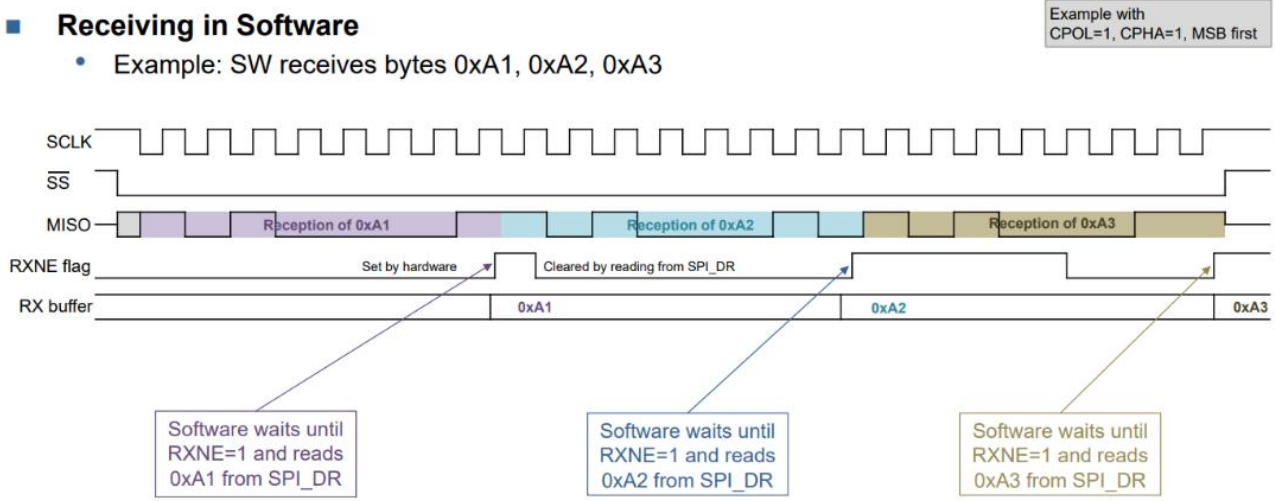
\includegraphics[width=\linewidth]{receiving_spi.png}
\end{concept}

\subsection{UART/I2C}

\begin{definition}{UART - Universal Asynchronous Receiver Transmitter}\\
    Connecting shift registers with diverging clock sources
    \begin{itemize}
        \item same target frequency
        \item different tolerances and divider ratios
        \item requires synchronization at start of each data item receiver
    \end{itemize}
    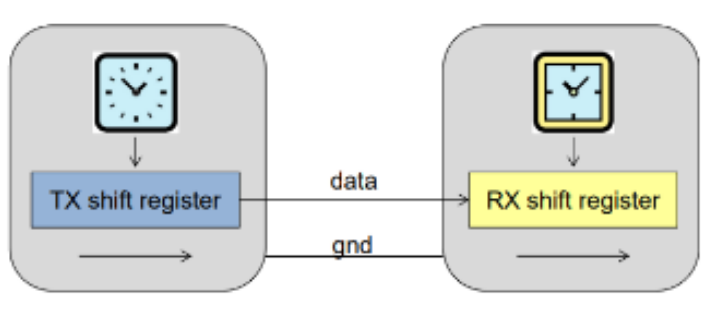
\includegraphics[width=\linewidth]{uart.png}
\end{definition}

\begin{concept}{UART Characteristics}
    \vspace{2mm}\\
    \textbf{synchronization}
    \begin{itemize}
        \item Each data item (5-8 bits) requires synchronization
    \end{itemize}
    \vspace{2mm}

    \textbf{Asynchronous data transfer}
    \begin{itemize}
        \item mismatch of clock frequencies in TX and RX
        \item requires overhead for synchronization $\rightarrow$ additional Bits
        \item requires effort for synchronization $\rightarrow$ additional Hardware
    \end{itemize}
    \vspace{2mm}

    \textbf{Advantages}
    \begin{itemize}
        \item Clock does not have to be transmitted
        \item transmission delays are automatically compensated
        \item no need for a common clock signal
    \end{itemize}
    \vspace{2mm}
    
    \textbf{on-board connections}
    \begin{itemize}
        \item signal levels are 3V or 5V with reference to ground
        \item off-board connections require strong output drivers
    \end{itemize}
\end{concept}

